\documentclass{report}
\usepackage{graphicx} % Required for inserting images
\usepackage{hyperref}
\usepackage{placeins}
\usepackage{minted}

\title{Bioinformatics Assignment}
\author{
1905065 Arnab Bhattacharjee\\
1905066 Abir Muhtasim\\
1905079 Salman Sayeed\\
1905095 Md. Raihan Sobhan\\
1905110 Md. Labid Al Nahiyan\\
}


\date{March 2024}

\begin{document}


\begin{titlepage}
    \centering

    \vspace*{2cm}
    {\LARGE \textbf{-----------------------------------------------------}}\\
    \vspace{1cm}
    {\LARGE \textbf{Bioinformatics Assignment \\ Motif Finding}}\\
    \vspace{0.5cm}
    {\large \textbf{CSE 463 : Introduction to Bioinformatics}}\\
    \vspace{1cm}
    {\LARGE \textbf{-----------------------------------------------------}}\\
    \vspace{0.5cm} 
    
    {\large \textbf{Supervisor: Dr. Muhammad Ali Nayeem}}\\
    \vspace{1cm}
    {\large \textbf{Department of Computer Science and Engineering}}\\
    \vspace{0.5cm}
    {\large \textbf{Bangladesh University of Engineering and Technology}}\\
    \vspace{2cm}
    
    \textbf{Group Members}
    
    \vspace{0.5cm}
    

        Arnab Bhattacharjee | 1905065\\
        Abir Muhtasim | 1905066\\
        Salman Sayeed | 1905079\\
        Md. Raihan Sobhan | 1905095\\
        Md. Labid Al Nahiyan | 1905110\\
            
    \vspace{2cm}
    \textbf{March 14, 2024}\\ 

\end{titlepage}
\clearpage

\tableofcontents

\chapter{Methods}
\section{Randomized Motif Search}
In randomized motif search, we first start with randomly selected k-mers in each string from DNA. Then we create a profile from those random k-mers. We keep on improving the motifs using the profile and improve the profile using the new motif. We run this algorithm many times at random starting positions and hope that we will get close to the optimum solution.

We have implemented randomized motif search in our code. The code is in the snipped below :
\begin{minted}[breaklines]{c++}
    #include<bits/stdc++.h>
using namespace std;

string find_random_motif(string str, int k, int n)
{
    int pos = rand() % (n - k);
    return str.substr(pos, k);
}

vector<string> find_profile_most_motifs(int t, int n, int k, string dna[], double profile[][100])
{
    double score, best_score;
    string temp;
    vector<string> profile_most_motifs;

    for(int i = 0; i < t; ++i)
    {
        best_score = 0;
        for(int j = 0; j < n-k; ++j)
        {
            score = 1;
            for(int pos = 0; pos < k; ++pos)
            {
                switch(dna[i][j+pos])
                {
                    case 'A':
                    case 'a': score *= profile[0][pos];
                            break;
                    case 'C':
                    case 'c': score *= profile[1][pos];
                            break;
                    case 'G':
                    case 'g': score *= profile[2][pos];
                            break;
                    case 'T':
                    case 't': score *= profile[3][pos];
                            break;
                }
            }
            if(score > best_score)
            {
                best_score = score;
                temp = dna[i].substr(j, k);
            }
        }
        profile_most_motifs.push_back(temp);
    }

    return profile_most_motifs;
}

void random_motif_search(int n, int t, int k, int it, string dna[])
{
    double profile[5][100];
    vector<string> profile_most_motifs, random_motifs;

    for(int i = 0; i < it; ++i)
    {
        profile_most_motifs.clear();
        random_motifs.clear();

        for(int j = 0; j < t; ++j)
            random_motifs.push_back( find_random_motif(dna[j], k, n) );

        int aa, cc, gg, tt;
        for(int j = 0; j < k; ++j)
        {
            aa = cc = gg = tt = 0;
            for(int l = 0; l < t; ++l)
            {
                switch(random_motifs[l][j])
                {
                    case 'A':
                    case 'a': ++aa;
                            break;
                    case 'C':
                    case 'c': ++cc;
                            break;
                    case 'G':
                    case 'g': ++gg;
                            break;
                    case 'T':
                    case 't': ++tt;
                            break;
                }
            }
            profile[0][j] = aa / (double) t;
            profile[1][j] = cc / (double) t;
            profile[2][j] = gg / (double) t;
            profile[3][j] = tt / (double) t;
        }

        profile_most_motifs = find_profile_most_motifs(t, n, k, dna, profile);
    }

    cout << "Random Motifs:" << endl;
    for(int i = 0; i < t; ++i)
        cout << random_motifs[i] << endl;
    cout << endl;

    char nuces[] = {'A', 'C', 'G', 'T'};
    cout << "Profile:" << endl;
    for(int i = 0; i < 4; ++i)
    {
        cout << nuces[i] << ": ";
        for(int j = 0; j < k; ++j)
            cout << fixed << setprecision(4) << profile[i][j] << " ";
        cout << endl;
    }
    cout << endl;

    cout << "Profile Most Motifs:" << endl;
    for(int i = 0; i < t; ++i)
        cout << profile_most_motifs[i] << endl;

    return;
}

int main()
{
    srand(time(NULL));
    int n, t, k, it;
    string dna[100];
    freopen("RMS_yst08r.txt","r",stdin);
    cin >> n >> t >> k >> it;
    for(int i = 0; i < t; ++i)
        cin >> dna[i];

    random_motif_search(n, t, k, it, dna);

    return 0;
}

\end{minted}



\section{Gibbs Sampling}
In Gibbs sampling for motif finding, the algorithm iteratively samples potential motif positions within each sequence while keeping the positions of the motifs in the other sequences fixed. It proceeds more slowly and chooses new l-mers at random increasing the odds that it will converge to the correct solution.
\\\\
\textbf{Working Procedure:}
\begin{enumerate}
    \item Randomly choose starting positions $s = (s_1,\ldots,s_t)$ and form the set of $l$-mers associated with these starting positions.
    \item Randomly choose one of the $t$ sequences.
    \item Create a profile $P$ from the other $t - 1$ sequences.
    \item For each position in the removed sequence, calculate the probability that the $l$-mer starting at that position was generated by $P$.
    \item Choose a new starting position for the removed sequence at random based on the probabilities calculated in step 4.
    \item Repeat steps 2-5 until there is no improvement.
\end{enumerate}

We have implemented randomized motif search in our code. The code is in the snipped below :
\\
\begin{minted}[breaklines]{python}
import random
from datetime import datetime

def symbolToNumber(symbol):
	if symbol == "A":
		return 0
	if symbol == "C":
		return 1
	if symbol == "G":
		return 2
	if symbol == "T":
		return 3

def numberToSymbol(x): 
	if x == 0:
		return "A"
	if x == 1:
		return "C"
	if x == 2:
		return "G"
	if x == 3:
		return "T"

def profileRandom(k, profile, text): 
    probs = [] 
    for i in range(0,len(text) - k +1): 
        prob = 1.0
        pattern = text[i:i+k] 
        for j in range(k):
            l = symbolToNumber(pattern[j]) 
            prob *= profile[l][j] 
        probs.append(prob) 
    r = myRandom(probs) 
    return r

def profileForm(motifs): 
	k = len(motifs[0]) 
	profile = [[1 for i in range(k)] for j in range(4)] 
	for x in motifs: 
		for i in range(len(x)): 
			j = symbolToNumber(x[i]) 
			profile[j][i] += 1 
	for x in profile: 
		for i in range(len(x)):
			x[i] = x[i]/len(motifs) 
	return profile

def consensus(profile):
	str = ""
	for i in range(len(profile[0])): 
		max = 0 
		loc = 0
		for j in range(4):
			if profile[j][i] > max: 
				loc = j 
				max = profile[j][i] 
		str+=numberToSymbol(loc) 
	return str

def score(motifs): 
	profile = profileForm(motifs)
	cons = consensus(profile)
	score = 0 
	for x in motifs: 
		for i in range(len(x)): 
			if cons[i] != x[i]: 
				score += 1 
	return score

def myRandom(dist): 
    s = 0.0
    for x in dist: 
        s+= x 
    i = random.random() 
    partial = 0.0
    for x in range(len(dist)): 
        partial += dist[x] 
        if partial/s >= i: 
            return x

def gibbsSampler(dna, k, t, n): 
    bestMotifs = []
    motifs = []
    for x in range(t): 
        i = random.randint(0, len(dna[x])-k) 
        motifs.append(dna[x][i:i+k]) 
    bestMotifs = motifs[:] 
    for i in range(n): 
        j = random.randint(0,t-1) 
        profile = profileForm(motifs[:j] + motifs[j+1:]) 
        r = profileRandom(k, profile, dna[j]) 
        motifs[j] = dna[j][r:r+k] 
        if score(motifs) < score(bestMotifs): 
            bestMotifs = motifs[:] 
    return bestMotifs

start = datetime.now()
with open("hm03.txt") as file:

    k, t, n = [int(x) for x in file.readline().split()] 
    dna = []
    for line in file:
        dna.append(line.rstrip()) 

best = gibbsSampler(dna, k, t, n) 
s = score(best)

for x in range(20): 
    sample = gibbsSampler(dna, k, t, n)
    if score(sample) < s: 
        s = score(sample) 
        best = sample[:] 
for b in best: 
	print(b)


end = datetime.now()
print("Runtime : ",end-start)
\end{minted}

\chapter{Software}
We ran all the files in both STREME and MEME_ChIP tools and the output was as follows : 
\section{STREME}
For this tool we just upload the DNA file that we want to find the motif in. But we need to provide the file in a different format. We need to have IDs before each line. After this, we simply upload our dna and an output file would be generated. We can view the HTML code and view this. Some of the outputs are as follows:
\FloatBarrier
\subsection{For file hm03.txt}
\begin{figure}[ht]
    \centering
    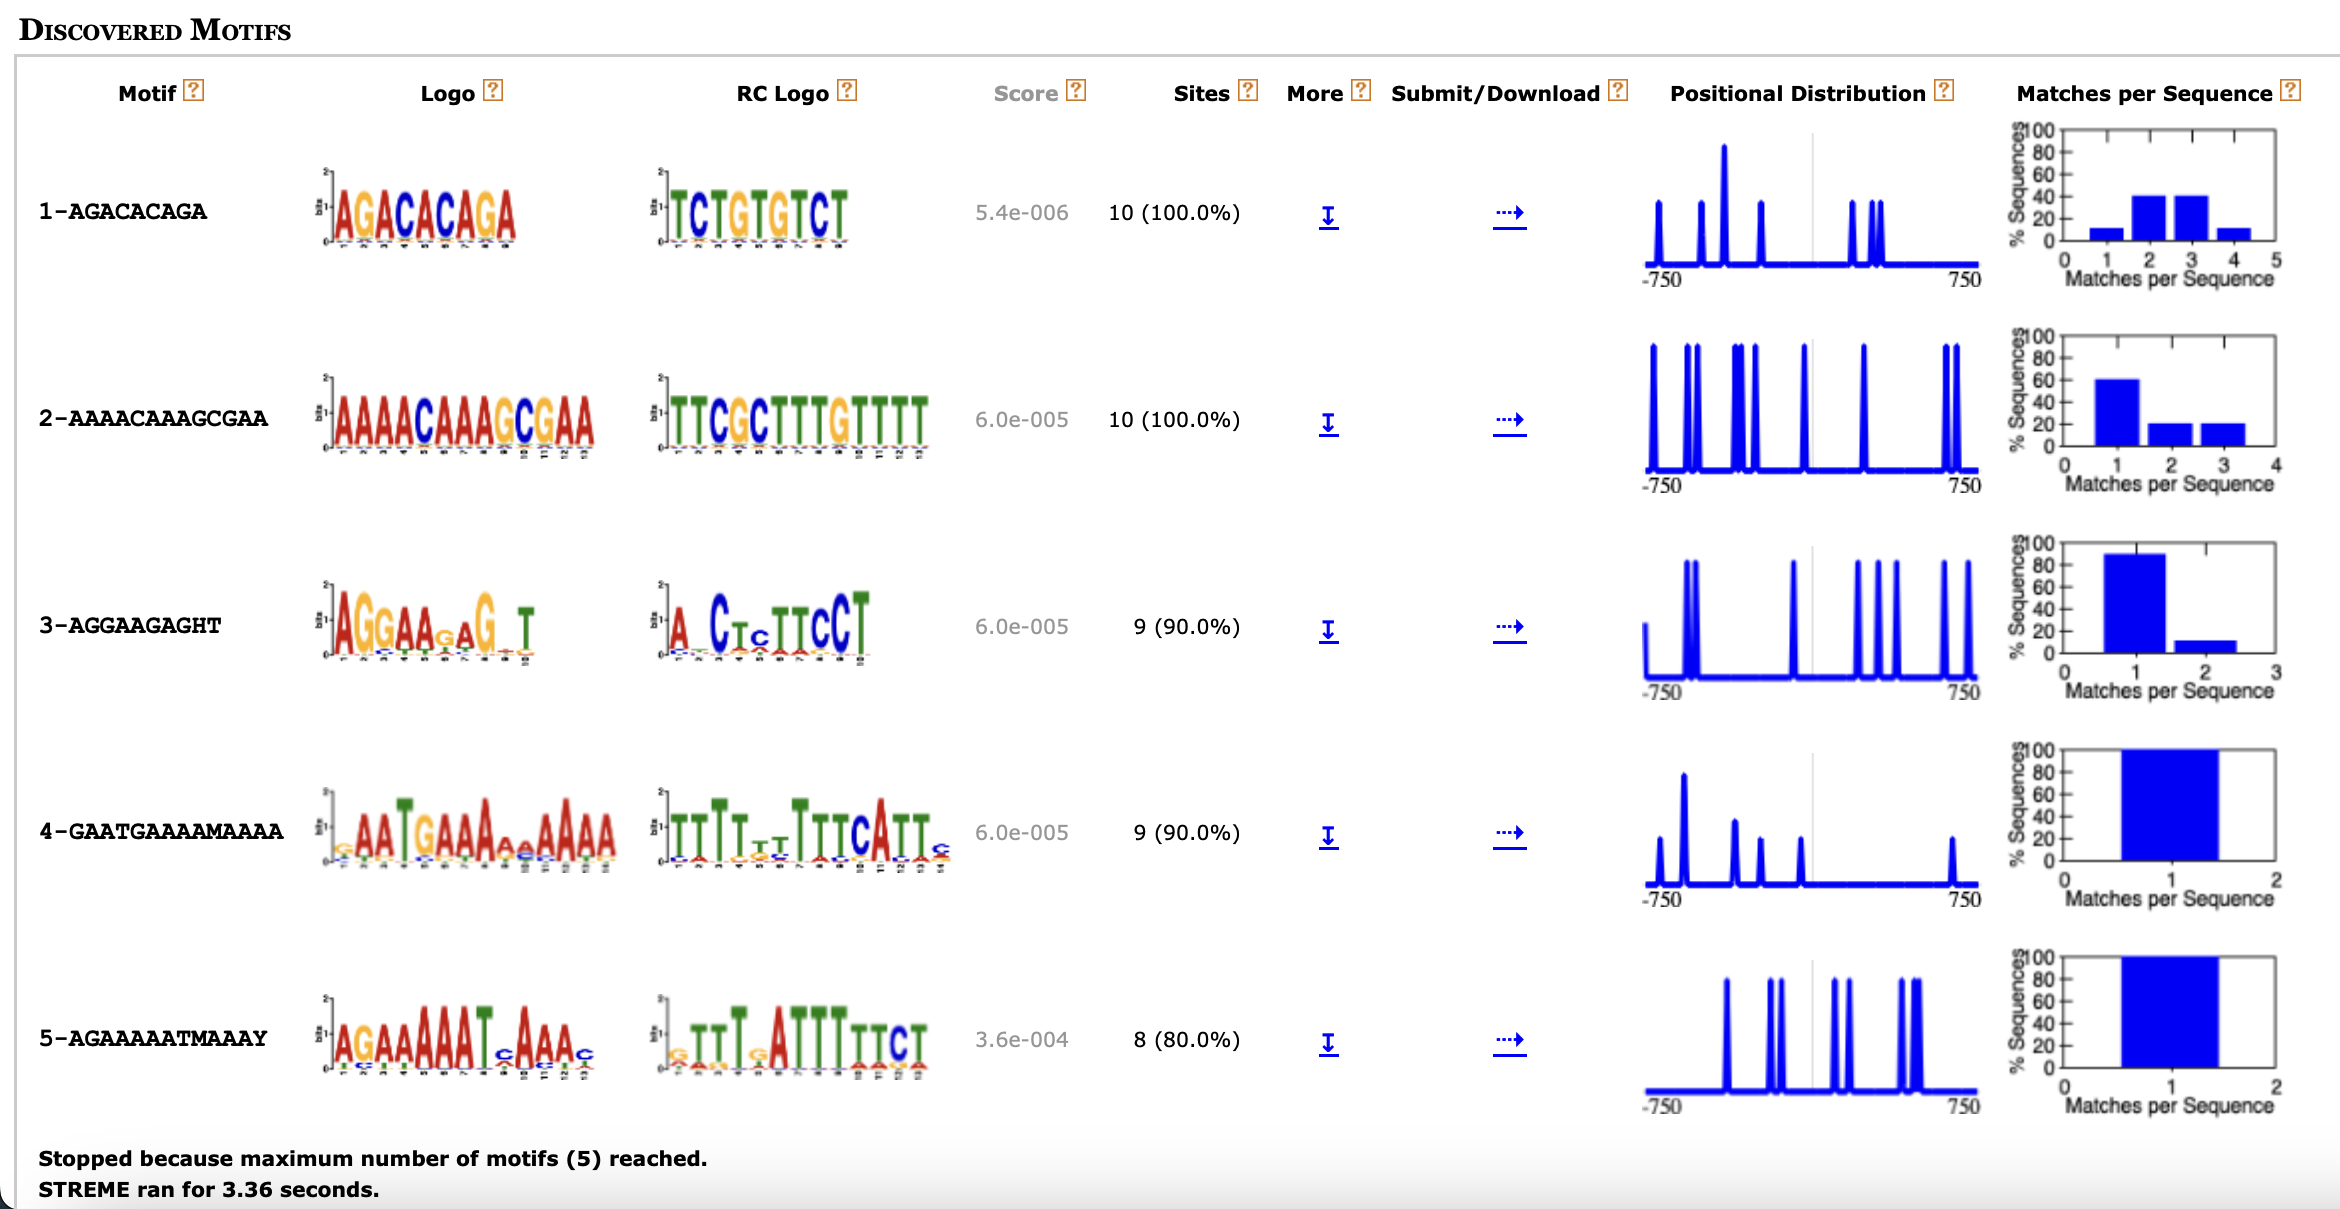
\includegraphics[width=0.9\textwidth]{STREME/STREME hm03.png} 
    \caption{Output for the file hm03.txt}
    \label{fig:ui2.4}
\end{figure}
\clearpage

\FloatBarrier
\subsection{For file yst04r.txt}
\begin{figure}[ht]
    \centering
    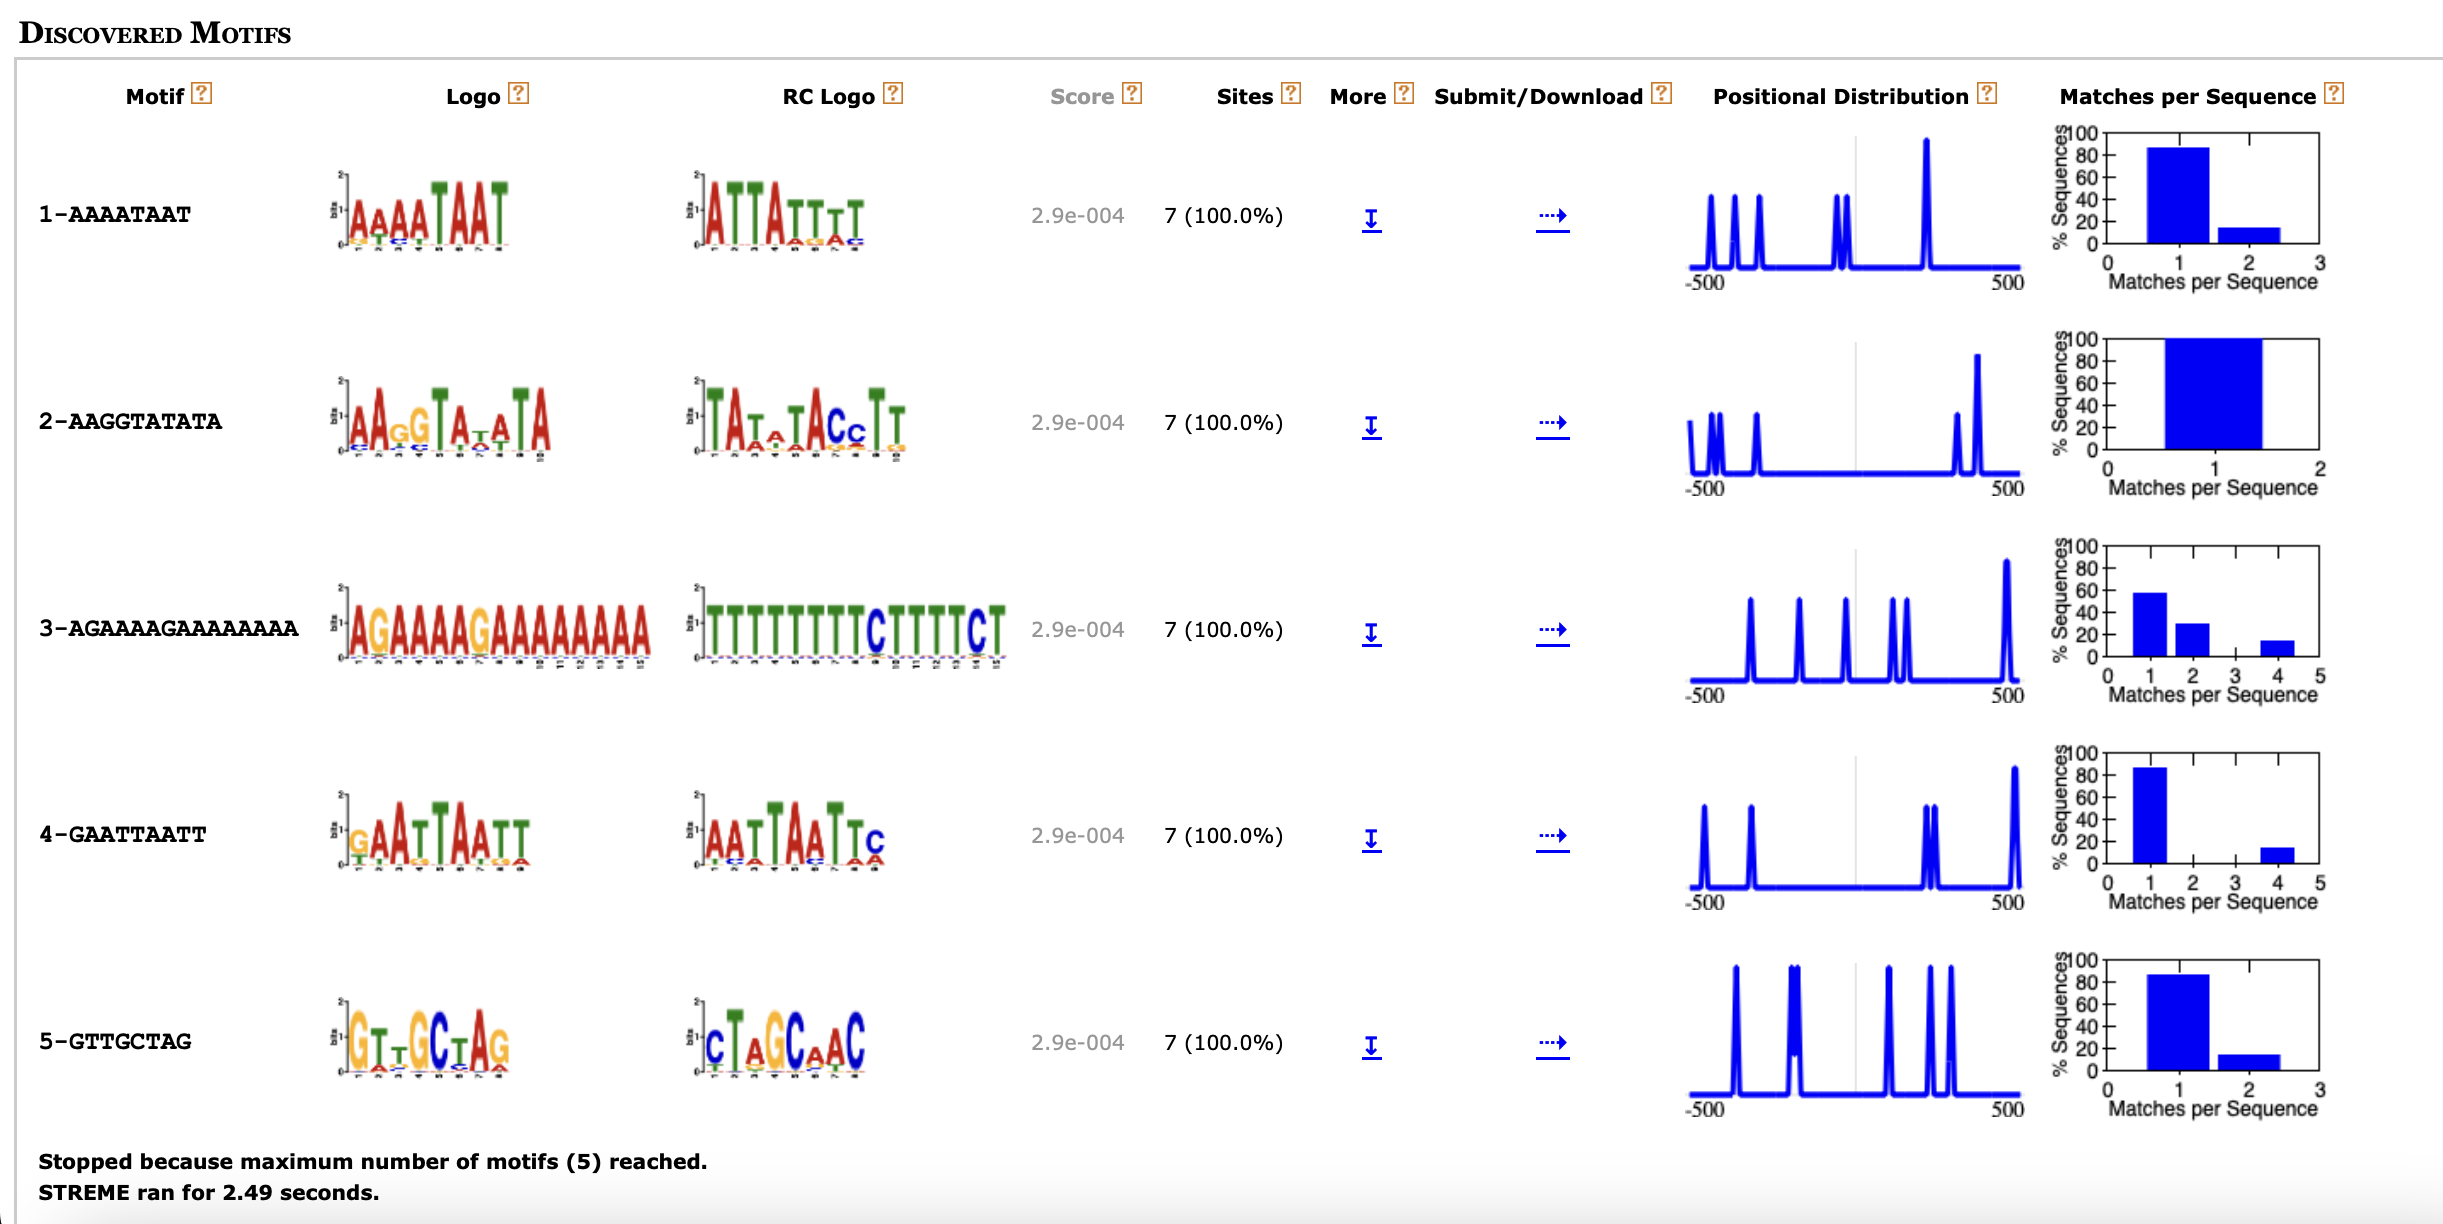
\includegraphics[width=0.9\textwidth]{STREME/STREME yst04r.png} 
    \caption{Output for the file yst04r.txt}
    \label{fig:ui2.4}
\end{figure}

\FloatBarrier
\subsection{For file yst08r.txt}

\begin{figure}[ht]
    \centering
    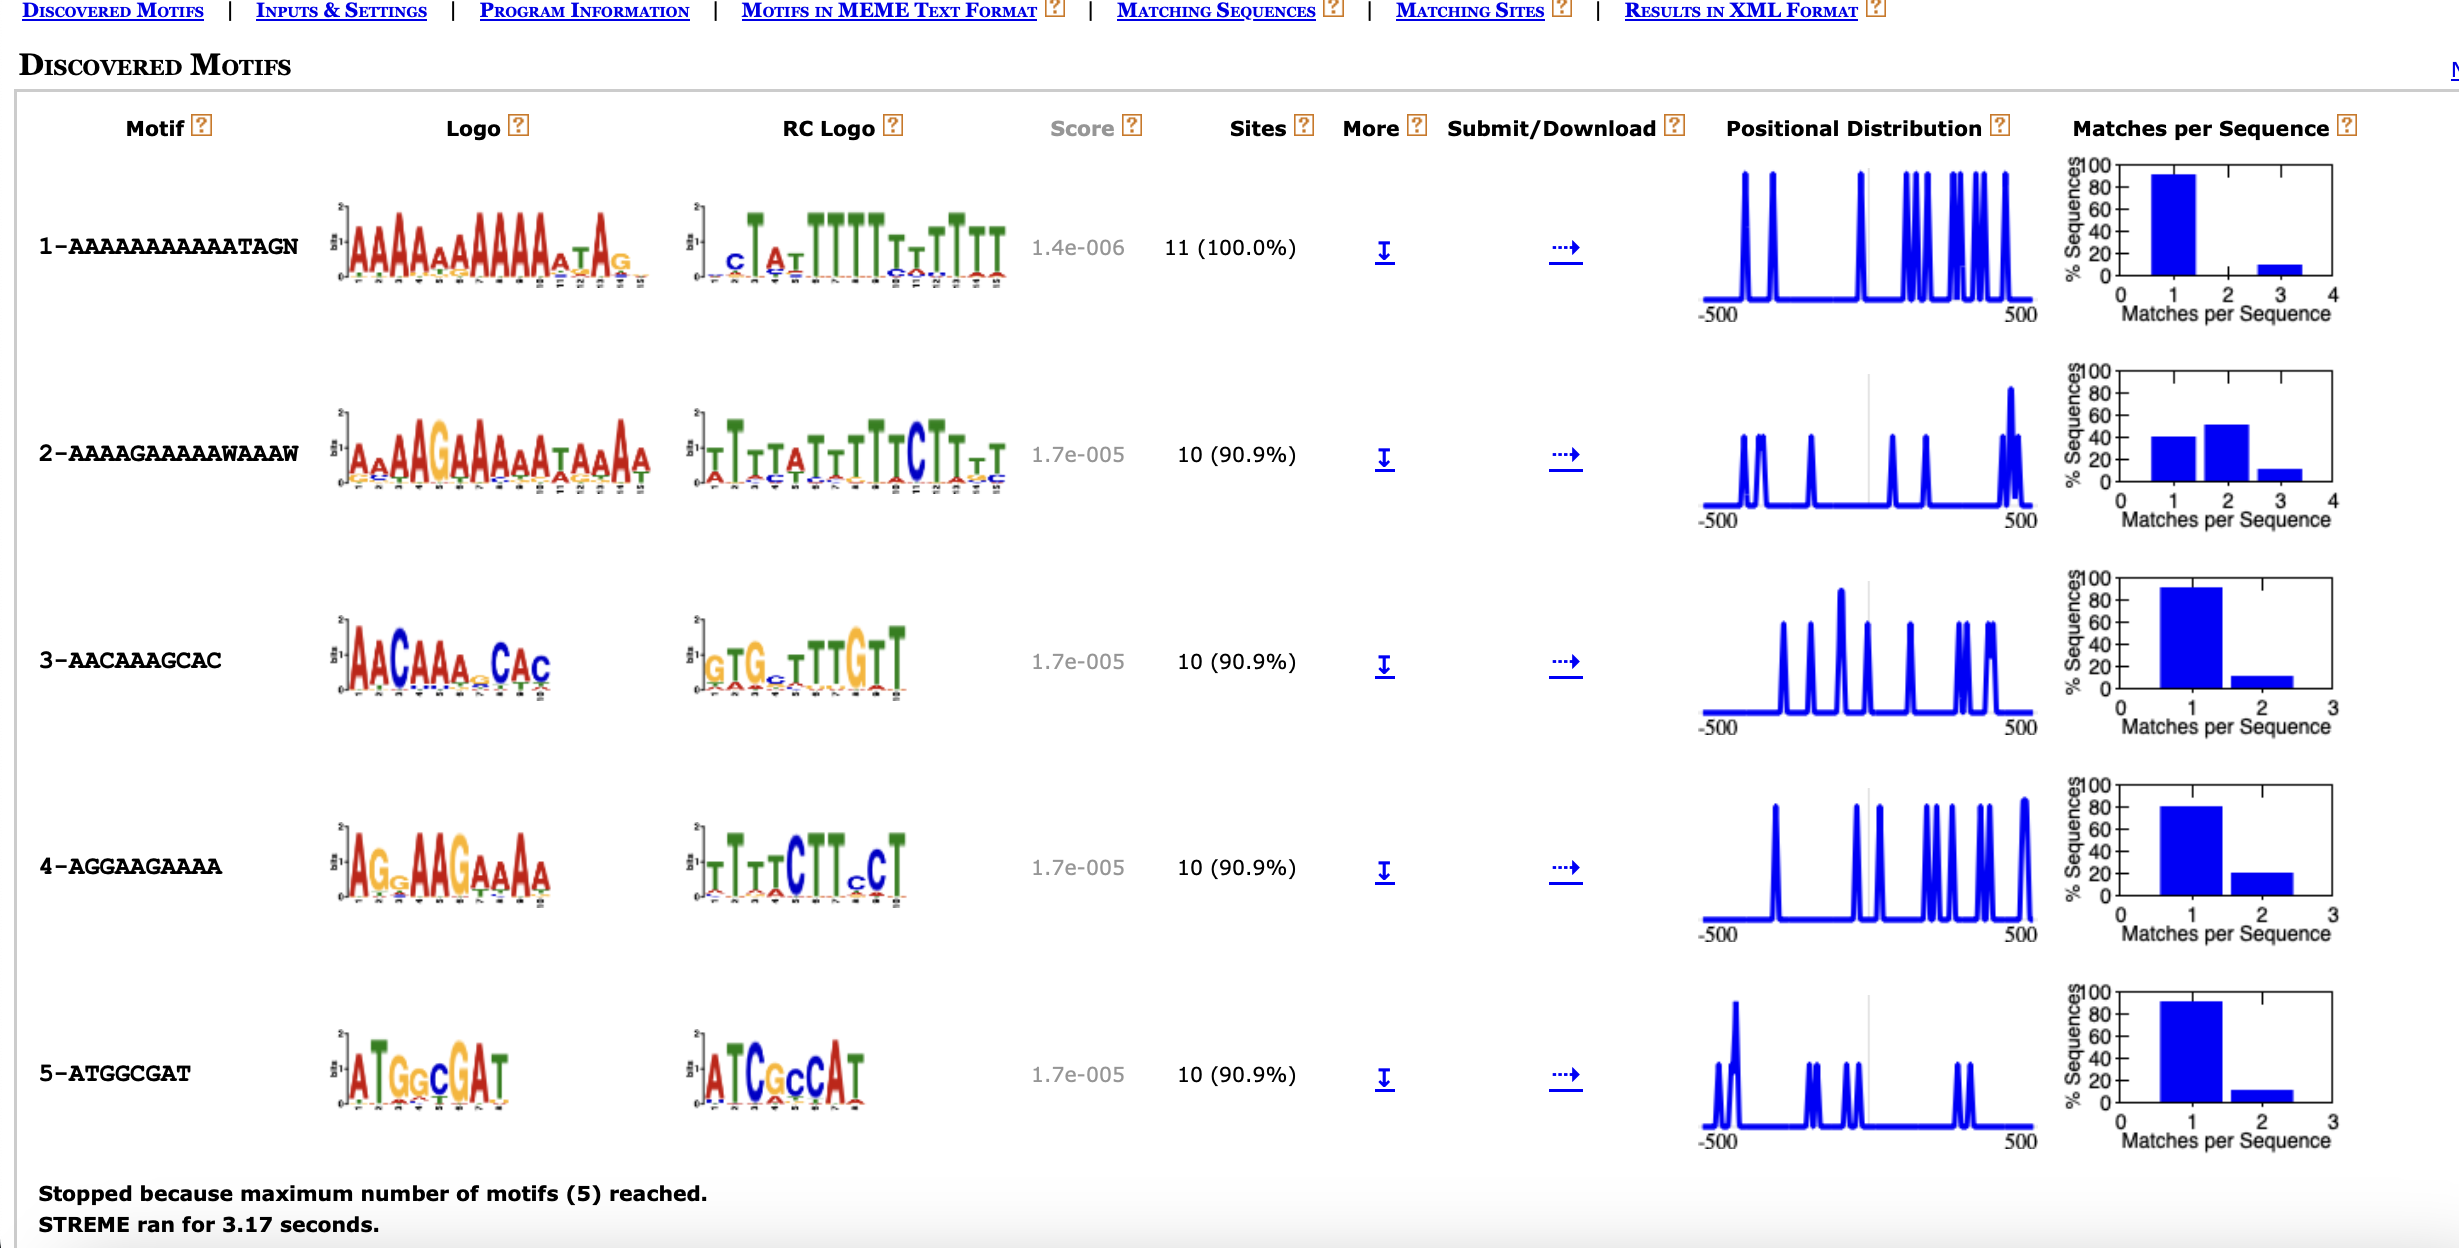
\includegraphics[width=0.9\textwidth]{STREME/STREME yst08r.png} 
    \caption{Output for the file yst08r.txt}
    \label{fig:ui2.4}
\end{figure}


\clearpage
\FloatBarrier
\section{MEME-ChIP}
For this tool we just upload the DNA file that we want to find the motif in. But we need to provide the file in a different format. We need to have IDs before each line. After this, we simply upload our dna and an output file would be generated. We can view the HTML code and view this. Some of the outputs are as follows:
\FloatBarrier
\subsection{For file hm03.txt}
\begin{figure}[ht]
    \centering
    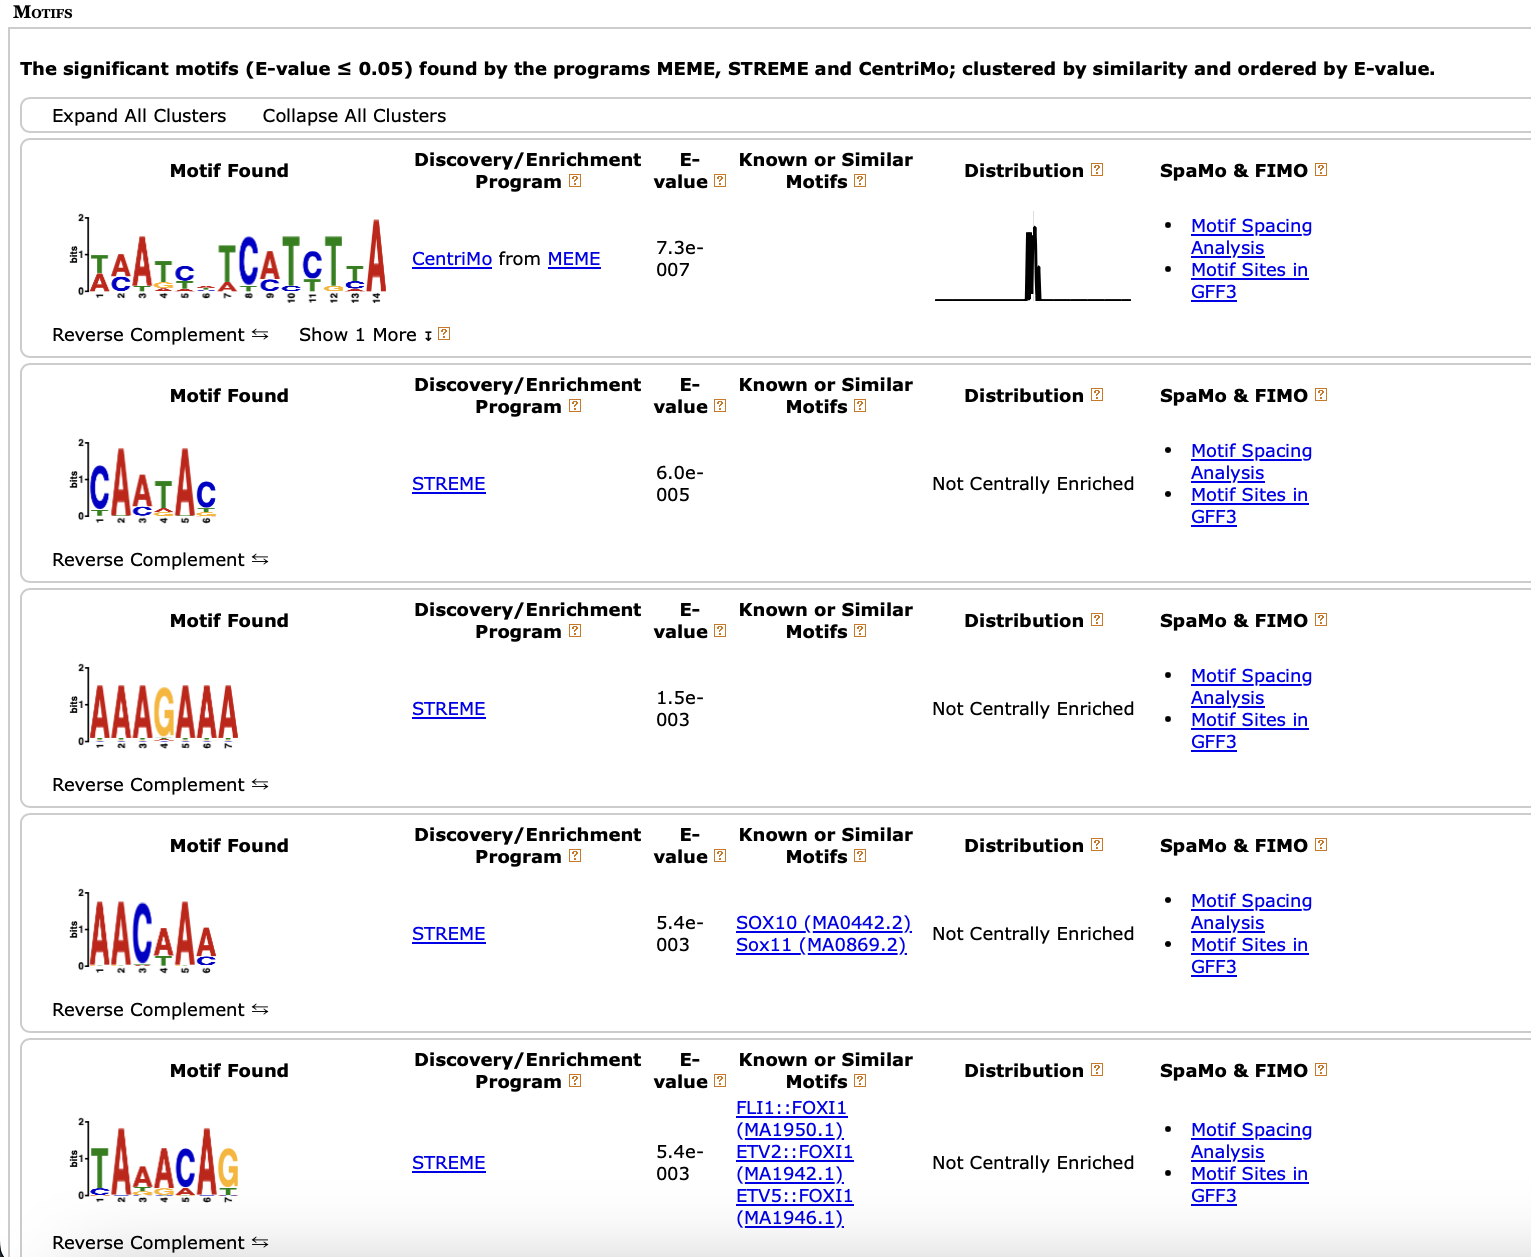
\includegraphics[width=0.9\textwidth]{MEME_CHIP/MEME_CHIP hm03.png} 
    \caption{Output for the file hm03.txt}
    \label{fig:ui2.4}
\end{figure}

\clearpage
\FloatBarrier
\subsection{For file yst04r.txt}
\begin{figure}[ht]
    \centering
    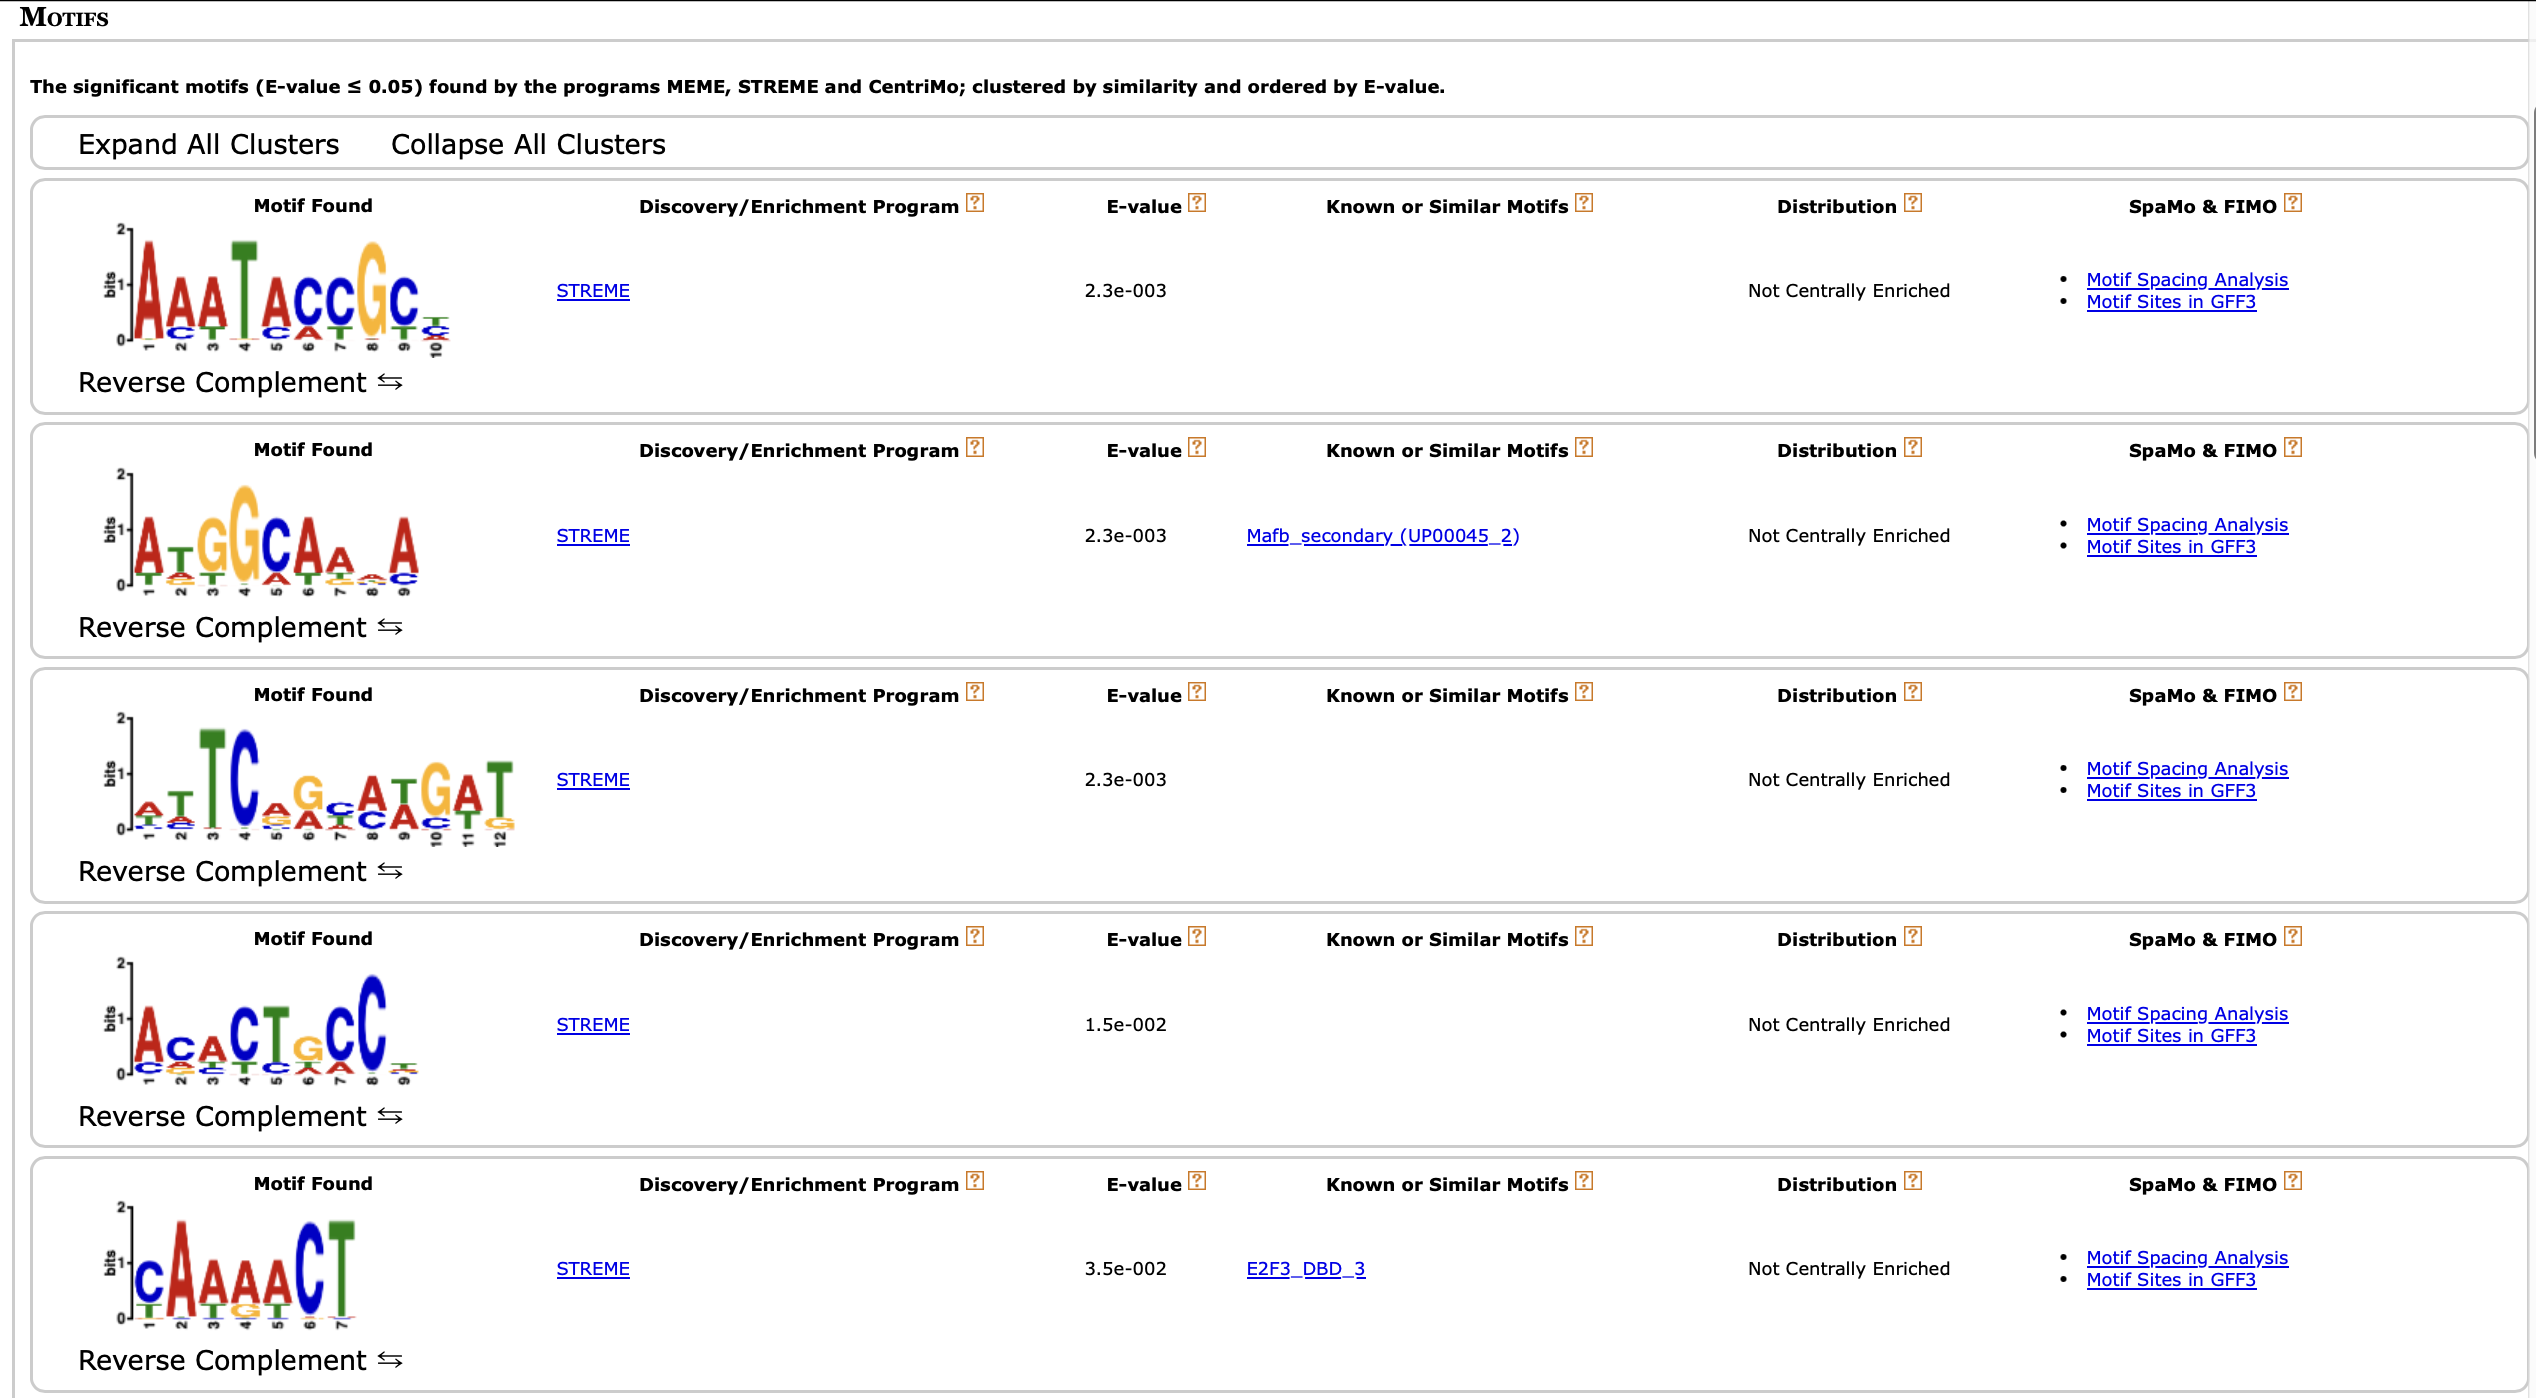
\includegraphics[width=0.9\textwidth]{MEME_CHIP/MEME_CHIP yst04r.png} 
    \caption{Output for the file yst04r.txt}
    \label{fig:ui2.4}
\end{figure}

\clearpage
\FloatBarrier
\subsection{For file yst08r.txt}
\begin{figure}[ht]
    \centering
    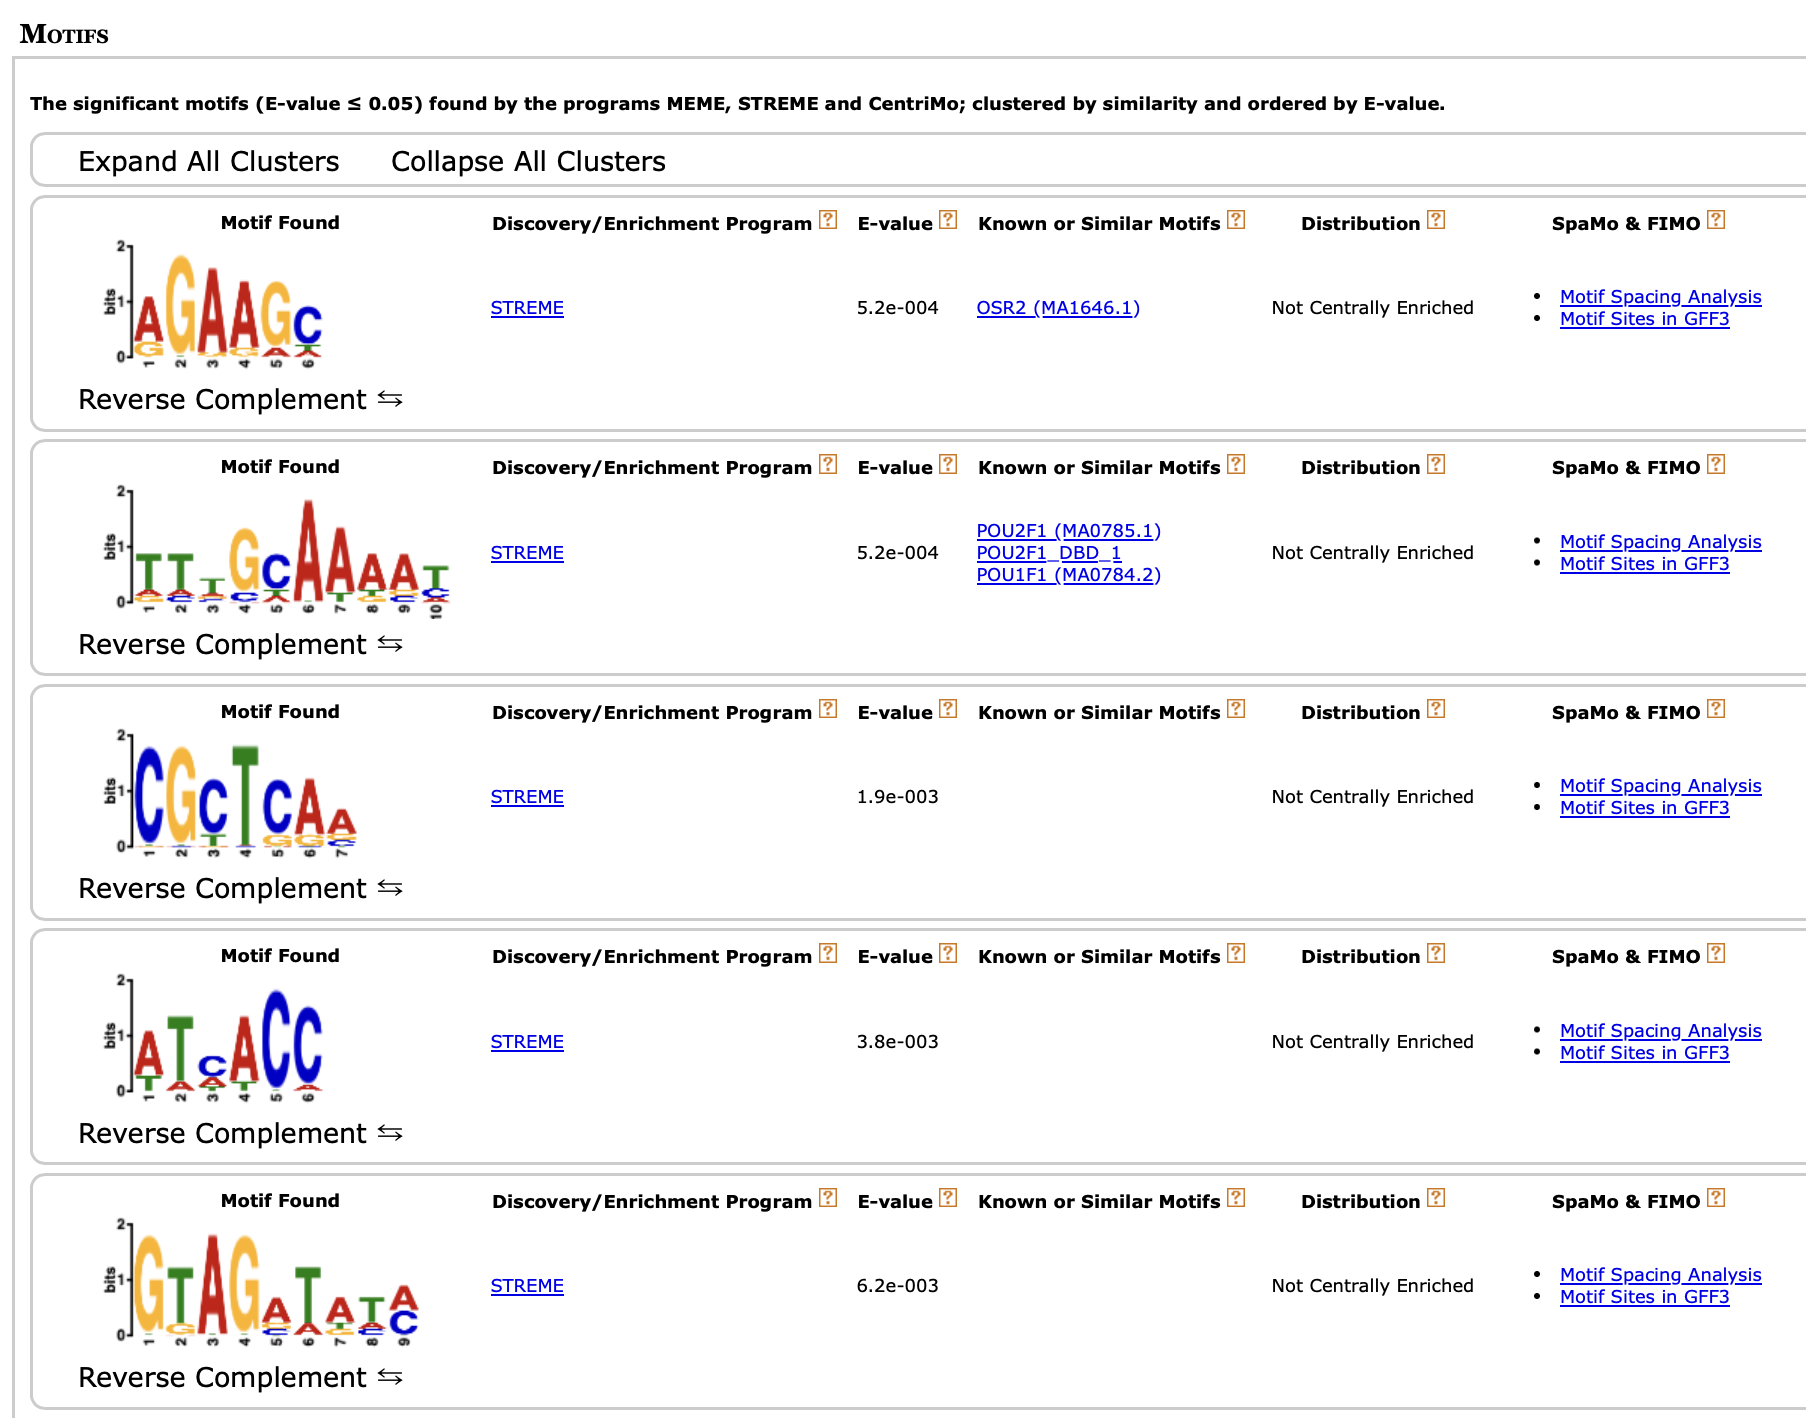
\includegraphics[width=0.9\textwidth]{MEME_CHIP/MEME_CHIP yst08r.png} 
    \caption{Output for the file yst08r.txt}
    \label{fig:ui2.4}
\end{figure}

\FloatBarrier

\clearpage
\section{Commands to run}

\section{STREME}
\subsection{For file hm03.txt}
streme --verbosity 1 --oc . --dna --totallength 4000000 --time 14400 --minw 8 --maxw 15 --thresh 0.05 --align center --p hm03.txt
\subsection{For file yst04r.txt}
streme --verbosity 1 --oc . --dna --totallength 4000000 --time 14400 --minw 8 --maxw 15 --thresh 0.05 --align center --p yst04r.txt
\subsection{For file yst08r.txt}
streme --verbosity 1 --oc . --dna --totallength 4000000 --time 14400 --minw 8 --maxw 15 --thresh 0.05 --align center --p yst08r.txt


\section{MEME-ChIP}
\subsection{For file hm03.txt}
meme-chip -oc . -time 240 -ccut 100 -dna -order 2 -minw 6 -maxw 15 -db db/motif_databases/MOUSE/uniprobe_mouse.meme -db db/motif_databases/JASPAR/JASPAR2022_CORE_vertebrates_non-redundant_v2.meme -db db/motif_databases/EUKARYOTE/jolma2013.meme -meme-mod zoops -meme-nmotifs 3 -meme-searchsize 100000 -streme-pvt 0.05 -streme-align center -streme-totallength 4000000 -centrimo-score 5.0 -centrimo-ethresh 10.0 hm03.txt
\subsection{For file yst04r.txt}
meme-chip -oc . -time 240 -ccut 100 -dna -order 2 -minw 6 -maxw 15 -db db/motif_databases/MOUSE/uniprobe_mouse.meme -db db/motif_databases/JASPAR/JASPAR2022_CORE_vertebrates_non-redundant_v2.meme -db db/motif_databases/EUKARYOTE/jolma2013.meme -meme-mod zoops -meme-nmotifs 3 -meme-searchsize 100000 -streme-pvt 0.05 -streme-align center -streme-totallength 4000000 -centrimo-score 5.0 -centrimo-ethresh 10.0 yst04r.txt
\subsection{For file yst08r.txt}
meme-chip -oc . -time 240 -ccut 100 -dna -order 2 -minw 6 -maxw 15 -db db/motif_databases/MOUSE/uniprobe_mouse.meme -db db/motif_databases/JASPAR/JASPAR2022_CORE_vertebrates_non-redundant_v2.meme -db db/motif_databases/EUKARYOTE/jolma2013.meme -meme-mod zoops -meme-nmotifs 3 -meme-searchsize 100000 -streme-pvt 0.05 -streme-align center -streme-totallength 4000000 -centrimo-score 5.0 -centrimo-ethresh 10.0 yst08r.txt


\chapter{Results}


\section{Experiment Configuration}
The tools provided us with motifs with size ranging from 8 to 15. We ran our algo for three of the input files for each of the values 8,10,12,15.\\


\section{Comparison}
\section{Randomized Motif Search}
We wrote a code following the pseudocode of the randomized motif search algorithm. Now we ran this code several times each time with a different motif length ranging from 8 to 15. These are some of the values that we received
\subsection{For file hm03.txt}
\textbf{When k=15, the output motifs were :}\\

Random Motifs:
ATCGGGTG\\
GTTTCTCA\\
TTGGGTGT\\\\
TTTTCTTT\\
CTTCCGGT\\
GGGACTGA\\
CTTCACTT\\
ATTGTGGA\\
AAGGCGAG\\
CGGGGCAG\\
\\
Profile:\\
A: 0.3000 0.1000 0.0000 0.1000 0.1000 0.0000 0.2000 0.3000\\
C: 0.3000 0.0000 0.1000 0.2000 0.5000 0.2000 0.1000 0.0000\\
G: 0.2000 0.2000 0.4000 0.5000 0.3000 0.4000 0.4000 0.3000\\
T: 0.2000 0.7000 0.5000 0.2000 0.1000 0.4000 0.3000 0.4000\\
\\
Profile Most Motifs:\\
CTGGCTGT\\
ATTGCTGG\\
TTTGCTGT\\
ATGGCTTT\\
CTGGCTGA\\
CTGGGTGA\\
CTTGCGGT\\
ATTGCTGT\\
CTGGCTTT\\

\\\\
\textbf{When k=10 the output was :} \\
Random Motifs:\\
TTATTCACTA\\
GTTGCAGCTT\\
AGAGCTGCTA\\
AAGATTATAG\\
CTCCCACTCG\\
AGAATGAGGC\\
TCCAAAAGTA\\
CCTGATGAAG\\
TTAAGGGAGT\\
GAAAATGAGG\\
\\
Profile:\\
A: 0.3000 0.2000 0.5000 0.5000 0.3000 0.3000 0.4000 0.3000 0.2000 0.3000\\
C: 0.2000 0.2000 0.2000 0.1000 0.3000 0.1000 0.1000 0.3000 0.1000 0.1000\\
G: 0.2000 0.2000 0.1000 0.3000 0.1000 0.2000 0.5000 0.2000 0.3000 0.4000\\
T: 0.3000 0.4000 0.2000 0.1000 0.3000 0.4000 0.0000 0.2000 0.4000 0.2000\\
\\
Profile Most Motifs:\\
ATAATAATTG\\
ATAATTAAAG\\
ATAAAAGCTG\\
TTAACTGAAG\\
ATAAATGGGG\\
TTAACTGAAG\\
AAAATTACTG\\
AAAATTGCTG\\
AGAATGAATG\\
GAAAATGAGG\\
\\
\textbf{When k=12 the output was :}\\
Random Motifs:\\
CACTAAACAGTCCTT\\
TCATGAATAATAATT\\
GCTTAAAAACCTAGA\\
ACAGAGAATTTGGGG\\
GACTGGTCACTCACC\\
TACTCACCCCATGGA\\
ACATACAATGCAGTA\\
TCTCATTATGCCTAC\\
CCCAGGTGCCCGCCC\\
CATCCTCCCCCAAAA\\
\\
Profile:\\
A: 0.2000 0.4000 0.3000 0.1000 0.5000 0.4000 0.5000 0.4000 0.4000 0.1000 0.1000 0.3000 0.4000 0.2000 0.4000\\
C: 0.3000 0.6000 0.4000 0.2000 0.2000 0.1000 0.2000 0.4000 0.3000 0.5000 0.5000 0.3000 0.2000 0.2000 0.3000\\
G: 0.2000 0.0000 0.0000 0.1000 0.3000 0.3000 0.0000 0.1000 0.0000 0.3000 0.0000 0.2000 0.3000 0.3000 0.1000\\
T: 0.3000 0.0000 0.3000 0.6000 0.0000 0.2000 0.3000 0.1000 0.3000 0.1000 0.4000 0.2000 0.1000 0.3000 0.2000\\

Profile Most Motifs:\\
CACTAAACAGTCATT\\
CACTATAAACTGTGA\\
GCTTAAAAACCTAGA\\
TACTAAACACTGAGA\\
GACTGGTCACTCACC\\
CCCCAAAAAGTAGGA\\
GACTAGTACCTGGGA\\
AACTGGTCACCCAGA\\
GCATGAACAGTGGGT\\
TCCTGGAACCTTCTT\\
\\
\textbf{When k=15 the output was :}\\
Random Motifs:\\
CACTGGACCCAGCTT\\
GTGCCTGACACAGGG\\
TCATGGCAAAGGTCT\\
TAGTTAATTAGTACC\\
TGTAACAATGAGCAC\\
ACCCGTAGTCCCGGC\\
TTTTATGCTGTATAA\\
GAGAAACAGGACTGT\\
TCAACAGGAATCCTC\\
CAATTCTGACAACAC\\

Profile:\\
A: 0.1000 0.4000 0.3000 0.3000 0.3000 0.3000 0.4000 0.4000 0.3000 0.4000 0.4000 0.3000 0.1000 0.3000 0.1000\\
C: 0.2000 0.3000 0.2000 0.2000 0.2000 0.2000 0.2000 0.2000 0.2000 0.3000 0.2000 0.3000 0.4000 0.2000 0.5000\\
G: 0.2000 0.1000 0.3000 0.0000 0.3000 0.2000 0.3000 0.3000 0.1000 0.3000 0.2000 0.3000 0.2000 0.3000 0.1000\\
T: 0.5000 0.2000 0.2000 0.5000 0.2000 0.3000 0.1000 0.1000 0.4000 0.0000 0.2000 0.1000 0.3000 0.2000 0.3000 \\
\\
Profile Most Motifs:\\
TAATCTAATGGGTGT\\
TAGAGAAATATGTCC\\
TCAACTAATAAGTCC\\
TAGTAAAAAAGACAC\\
TCATCTGAAGAAGGC\\
TCGACTGATAAACGC\\
GAGTATAGTCTGTGT\\
TCATTCAACAAATAT\\
CACCAAAATAAACAT\\
GCATATAGAAGGCAC\\


\subsection{For file yst04r.txt}
\textbf{When k=8, the output motifs were :}\\
Random Motifs:\\
ACAGATCA\\
AATACATT\\
CCACACCA\\
ATAAAAAA\\
AAACACTA\\
CACGCCTT\\
CCTGGTCA\\
\\
Profile:\\
A: 0.5714 0.4286 0.5714 0.2857 0.5714 0.2857 0.1429 0.7143\\
C: 0.4286 0.4286 0.1429 0.2857 0.2857 0.4286 0.4286 0.0000\\
G: 0.0000 0.0000 0.0000 0.4286 0.1429 0.0000 0.0000 0.0000\\
T: 0.0000 0.1429 0.2857 0.0000 0.0000 0.2857 0.4286 0.2857\\

Profile Most Motifs:\\
AAAGAACA\\
AAAGATTA\\
AAAAACTA\\
CAAGACTA\\
AAAAACCA\\
AAACACTA\\
AAAGATTA\\
\textbf{When k=10, the output motifs were :}\\
Random Motifs:\\
TGGTCTTTTC\\
TGAGGACCTT\\
AAAAACACCA\\
GTTACAATAT\\
AGAAAAATAC\\
TTTGACATTG\\
TAAAATTGAT\\
\\
Profile:\\
A: 0.2857 0.2857 0.5714 0.5714 0.5714 0.4286 0.5714 0.0000 0.4286 0.1429\\
C: 0.0000 0.0000 0.0000 0.0000 0.2857 0.2857 0.1429 0.2857 0.1429 0.2857\\
G: 0.1429 0.4286 0.1429 0.2857 0.1429 0.0000 0.0000 0.1429 0.0000 0.1429\\
T: 0.5714 0.2857 0.2857 0.1429 0.0000 0.2857 0.2857 0.5714 0.4286 0.4286\\
\\
Profile Most Motifs:\\
TGAAACTTAC\\
TAAGACTTTT\\
TATAAAATTC\\
TGTACAATAT\\
AGAAAAATTT\\
TGAAAAATTC\\
AAAACAATAT\\
\textbf{When k=12, the output motifs were :}\\
Random Motifs:\\
TTAATTTTTTTTTCT\\
AAGAGAGAAGACCCA\\
CTGTCTCGAGGGTGC\\
TGTAGCCCTAGACTT\\
AGAAAGCATACTATA\\
CAAGTGTCGACGCTG\\
AAATGTGTTCCGCAC\\
\\
Profile:
A: 0.4286 0.4286 0.5714 0.5714 0.1429 0.1429 0.0000 0.2857 0.2857 0.4286 0.1429 0.1429 0.1429 0.1429 0.2857\\
C: 0.2857 0.0000 0.0000 0.0000 0.1429 0.1429 0.4286 0.2857 0.0000 0.1429 0.4286 0.1429 0.5714 0.2857 0.2857\\
G: 0.0000 0.2857 0.2857 0.1429 0.4286 0.2857 0.2857 0.1429 0.1429 0.2857 0.2857 0.4286 0.0000 0.1429 0.1429\\
T: 0.2857 0.2857 0.1429 0.2857 0.2857 0.4286 0.2857 0.2857 0.5714 0.1429 0.1429 0.2857 0.2857 0.4286 0.2857\\

Profile Most Motifs:\\
CTAATTCGTAGTTTT\\
AATAATCCTACGTTA\\
TAATGTCTTACTTCT\\
TAAAGTCCAATGCTA\\
AGAAAGCATACTATA\\
CTAATTGATACATCT\\
CAAAGTTATTCTCTA\\
\textbf{When k=15, the output motifs were :}\\
Random Motifs:\\
AAGTAATTATCTACT\\
AAATCTATAACTACA\\
GATCAATCAGTACTA\\
CTAAAGGAAAAAATT\\
TTATCTACTGATCCG\\
AAACGAAGGCTATCG\\
TATTATTCTCTCTTG\\
\\
Profile:\\
A: 0.4286 0.7143 0.5714 0.1429 0.5714 0.4286 0.4286 0.1429 0.5714 0.2857 0.2857 0.4286 0.4286 0.0000 0.2857\\
C: 0.1429 0.0000 0.0000 0.2857 0.2857 0.0000 0.0000 0.4286 0.0000 0.2857 0.2857 0.1429 0.2857 0.5714 0.0000\\
G: 0.1429 0.0000 0.1429 0.0000 0.1429 0.1429 0.1429 0.1429 0.1429 0.2857 0.0000 0.0000 0.0000 0.0000 0.4286\\
T: 0.2857 0.2857 0.2857 0.5714 0.0000 0.4286 0.4286 0.2857 0.2857 0.1429 0.4286 0.4286 0.2857 0.4286 0.2857\\

Profile Most Motifs:\\
AAGTAATTATCTACT\\
AAATCTATAACTACA\\
TTATAAACATCAACA\\
AATTAAAGTCCAATG\\
TATTAATCAAATTTA\\
AAATATTTGACATTG\\
AAATAAACAATCACA\\

\\


\subsection{For file yst08r.txt}
\textbf{When k=8, the output motifs were :}\\
Random Motifs:\\
TTCCACTA\\
TTGGTTAC\\
TCTGTTAG\\
ATCCTTTG\\
TCCTCGTT\\
GTTCTACT\\
ATGCTAAA\\
ACGAGAAA\\
CGCTCAAA\\
ATACATAT\\
AGTTATAA\\
\\
Profile:\\
A: 0.4545 0.0000 0.0909 0.0909 0.2727 0.3636 0.6364 0.4545\\
C: 0.0909 0.2727 0.3636 0.4545 0.1818 0.0909 0.0909 0.0909\\
G: 0.0909 0.1818 0.2727 0.1818 0.0909 0.0909 0.0000 0.1818\\
T: 0.3636 0.5455 0.2727 0.2727 0.4545 0.4545 0.2727 0.2727\\
\\
Profile Most Motifs:\\
TTTCATAA\\
ATCCAAAA\\
TTCCTTAA\\
ATTCTTAA\\
TTTTTTAA\\
TTCCAAAA\\
ATCTTTAA\\
ATGTTTAA\\
TTTCAAAA\\
ATCCTTTA\\
ATTCTAAA\\
\textbf{When k=10, the output motifs were :}\\
Random Motifs:\\
ATCGAAGCCG\\
TGGTTCATTA\\
CTCTCCTTGC\\
AATGGAAAAA\\
GGGCGACGAA\\
AGCTACAGTT\\
CTTTCGATGA\\
GTTCCTTGAG\\
CCGCCGACGA\\
AAAACCCAGA\\
AGGATGAGCC\\

Profile:\\
A: 0.4545 0.1818 0.0909 0.1818 0.1818 0.2727 0.5455 0.1818 0.2727 0.5455\\
C: 0.2727 0.0909 0.2727 0.2727 0.4545 0.3636 0.1818 0.1818 0.1818 0.1818\\
G: 0.1818 0.3636 0.3636 0.1818 0.1818 0.2727 0.0909 0.3636 0.3636 0.1818\\
T: 0.0909 0.3636 0.2727 0.3636 0.1818 0.0909 0.1818 0.2727 0.1818 0.0909\\
\\
Profile Most Motifs:\\
ATCTCCACGA\\
CGTTCCAAAA\\
ATGTGCAAGA\\
ATTTCCAAGA\\
ATGGCAACGA\\
CTGTCCAGGA\\
CTTTCGATGA\\
ATGACGAGAA\\
CTGGCAAGGA\\
AGGGCCAGAA\\
ATTTCCAAAA\\
\textbf{When k=12, the output motifs were :}\\
Random Motifs:\\
AGAGTGCATATC\\
ACAAACAATGGC\\
TGAAGGCCAAAT\\
AGTGATTTCCTT\\
ACGCTTGCTTTG\\
AGACGAGGTTTG\\
CATATTACATAT\\
TTGAGCTACCCT\\
TACACTGTAATG\\
ACTTCCCATACT\\
TTTGTATTCTTT\\

Profile:\\
A: 0.5455 0.1818 0.3636 0.4545 0.1818 0.1818 0.1818 0.3636 0.2727 0.3636 0.1818 0.0000\\
C: 0.0909 0.2727 0.0909 0.1818 0.1818 0.2727 0.2727 0.2727 0.2727 0.1818 0.1818 0.1818\\
G: 0.0000 0.3636 0.1818 0.2727 0.2727 0.1818 0.2727 0.0909 0.0000 0.0909 0.0909 0.2727\\
T: 0.3636 0.1818 0.3636 0.0909 0.3636 0.3636 0.2727 0.2727 0.4545 0.3636 0.5455 0.5455\\

Profile Most Motifs:\\
TCTAGCTATTTT\\
TTAATTTTTTTT\\
ACTATTTTTTTT\\
TGAATTATTTTT\\
ACAAGCTTATTT\\
AGTAACCTTTTT\\
AAAATTTTTTTT\\
TCTAGTGCTATT\\
TCAAGTGCATTT\\
TTAATTTTTTTT\\
AATATTTTTCTT\\
\textbf{When k=15, the output motifs were :}\\
Random Motifs:\\
GCCAAAAACTGATAT\\
CAACTAATACTATAA\\
ACACACCCCGCGTTT\\
GCAACGGCGGGATTC\\
CGAAAAAGCCAATCT\\
GACCAATGGCAGAGA\\
CTCCGCGCATCGCCG\\
TCCCCTGCCGGCTGT\\
TCAAAACGCTCAAAA\\
CAAGGGGGTGGTTTA\\
ATCGTTTACCAATGT\\

Profile:\\
A: 0.1818 0.2727 0.5455 0.3636 0.4545 0.4545 0.2727 0.1818 0.1818 0.0000 0.2727 0.5455 0.1818 0.2727 0.3636\\
C: 0.3636 0.4545 0.4545 0.4545 0.1818 0.1818 0.1818 0.3636 0.5455 0.3636 0.2727 0.0909 0.0909 0.1818 0.0909\\
G: 0.2727 0.0909 0.0000 0.1818 0.1818 0.1818 0.3636 0.3636 0.1818 0.3636 0.3636 0.2727 0.0000 0.2727 0.0909\\
T: 0.1818 0.1818 0.0000 0.0000 0.1818 0.1818 0.1818 0.0909 0.0909 0.2727 0.0909 0.0909 0.7273 0.2727 0.4545\\

Profile Most Motifs:\\
GCCAAAAACTGATAT\\
ACAAAAGCGGGATGA\\
ACACACCCCGCGTTT\\
AAAAATAGCTAATTT\\
CGAAAAAGCCAATCT\\
TTCCTAAGCCAATCT\\
CGAAAAAGGCAATAA\\
ACAAATTACCCATAA\\
AAAAAAAGCGCATGC\\
TAAAGATGCCGATTT\\
CAAAGGAGCCTATAT\\

\section{Gibbs Sampler}
We wrote a code following the pseudocode of the gibbs-sampler algorithm. Now we ran this code several times each time with a different motif length ranging from 8 to 15. These are some of the values that we received.
\subsection{For file hm03.txt}
\textbf{When k=8, the output motifs were :} 
\begin{itemize}
    \item AAAAAAAA
    \item AAAAAAAA
    \item AAAATAAA
    \item AAAAAAAA
    \item AAACAAAG
    \item AAAAAAAA
    \item AAGAACAA
    \item AAAATAAA
    \item AAAAAAAA
    \item ACACAAAA
\end{itemize}\\
The running time for this code was 2:02min\\
\textbf{When k=10, the output motifs were : }

\begin{itemize}
    \item AAAAAAAATA
    \item AAACAAAATA
    \item AAACAAAATA
    \item AAAAGACACA
    \item AAAGCAAACA
    \item AAAAAAAACA
    \item ACAATAAACA
    \item AAATAAAACA
    \item AAAAAAAAAA
    \item ACAAAAATCA
    
\end{itemize}\\
The running time for this code was 2:25min\\
\textbf{When k=12, the output motifs were : }

\begin{itemize}
    \item AAAAAAAATAAA
    \item AAACAAAATAAA
    \item AAACAAAATAAA
    \item AGAAAAAATAAT
    \item AAAAGAAGTAAC
    \item AAAAATAAAAAA
    \item AGACACAATAAA
    \item AAGTAAAATAAA
    \item AAAAAAAAAAAA
    \item AACAAAAATCAA
\end{itemize}\\
The running time for this code was 2:42min\\
\textbf{When k=15, the output motifs were : }
\begin{itemize}
    \item AGCAAAAAAAATAAA
    \item AGCAAACAAAATAAA
    \item AGCAAACAAAATAAA
    \item GGAAAAAAATATGAA
    \item TGGAAAAGAAGTAAC
    \item ACAAAAATAAAAAAA
    \item AGAAGACACAATAAA
    \item AGTAAGTAAAATAAA
    \item AAAAAAAAAAAAAAA
    \item TGAACAAAAATCAAA
\end{itemize}
The running time for this code was 3:12min\\







\subsection{For file yst04r.txt}
\textbf{When k=8, the output motifs were : }
\begin{itemize}
    \item TTTTTTTT
    \item TTTTTCTT
    \item TTTTTTTA
    \item TTTTTTTT
    \item TTTTGTTT
    \item TTTTTTTT
    \item TTTTTTTT
\end{itemize}
The running time for this code was 1:10min\\

\textbf{When k=10, the output motifs were : }
\begin{itemize}
    \item TTTTTTTTCT
    \item ATTCTTTTCT
    \item TTTTTTTTAT
    \item TTTTTTTTCT
    \item TTATTTTACT
    \item TTTTTTTTCT
    \item TTTTTTTTTT

\end{itemize}
The running time for this code was 1:37min\\

\textbf{When k=12, the output motifs were : }
\begin{itemize}
    \item TTTTTTTCTTTC
    \item TATTTTTCTTTT
    \item TATTTTTTTTAT
    \item TTTTTTTCTTTT
    \item TATTTTACTTCT
    \item TATTTTTCTTTT
    \item TATTTTTTTTTT
\end{itemize}
The running time for this code was 1:54min\\

\textbf{When k=15, the output motifs were : }
\begin{itemize}
    \item TTCTTTTTCTCTTTT
    \item ATATTTTTCTTTTTA
    \item TTATTTTTATATTTA
    \item TTTTTTTTCTTTTCT
    \item TTATTTTACTTCTTT
    \item TTATTTTTCTTTTCT
    \item TTATTTTTTTTTTGT

\end{itemize}
The running time for this code was 2:16min\\

\subsection{For file yst08r.txt}
\textbf{When k=8, the output motifs were : }
\begin{itemize}
    \item TCTTTTGT
    \item TTTTTTTT
    \item TTTTTTTT
    \item TTTTTTTT
    \item TTTTTTTT
    \item TATTTTTT
    \item TTTTTTTT
    \item TTTTTTTT
    \item TTTTTTCT
    \item TTTTTTTT
    \item TTCTTTTT
\end{itemize}
The running time for this code was 0:37min\\
\subsection{For file yst08r.txt}
\textbf{When k=10, the output motifs were : }
\begin{itemize}
    \item TCTTTTGTTT
    \item TTTTTATTTT
    \item TTTTTTTTTT
    \item TTTTTTTTTT
    \item TTTTTTGTTT
    \item TTTTTATTTT
    \item TTTTTTTTTT
    \item TTTTTTTTTT
    \item TTTTTTCTAT
    \item TTTTTTCTTT
    \item TTTTTTGTTT
\end{itemize}
The running time for this code was 1:47min\\
\subsection{For file yst08r.txt}
\textbf{When k=12, the output motifs were : }
\begin{itemize}
    \item TATTTTACTTCT
    \item TATTTTATTTTT
    \item TATTTTTTTTTT
    \item TATTTTTTTTTT
    \item TATCTTTTTTTC
    \item TATTTTTTATTT
    \item AATTTTTTTTTT
    \item TATTTTTTTTTT
    \item TATCTTTTATGT
    \item TAATTTTTTTTT
    \item TATTTTTCTTTT
\end{itemize}
The running time for this code was 1:54min\\
\subsection{For file yst08r.txt}
\textbf{When k=15, the output motifs were : }
\begin{itemize}
    \item TTTACTTCTTTCTTG
    \item TTTATTTTTCTTTTC
    \item TTTATTTACCTATCT
    \item TTTATTATTCTCTCT
    \item TTTATTTCTTTCTTT
    \item TATACTTTTCTATTT
    \item TTGATTTTTTTCTCT
    \item TCTATTTTTCTCTCT
    \item TTTATTTCTCTCTCT
    \item TTTCTTTTTCTCTTT
    \item AATATTTTTCTTTTT
\end{itemize}
The running time for this code was 2:26min\\
\chapter{Conclusion}
We can conclude by saying that both the tools perform exceptionally well when it comes to estimating motifs in a provided DNA. The algorithms that we have implemented i.e. Randomized Motif Search and Gibbs Sampling also produced convincing outputs. However, the RMS algoritm needs to be run multiple times for ensuring close to accurate answers.

\chapter{Reference}

\section{Method 1 : Randomized Motif Search}
\href{https://bioinformatics.stackexchange.com/questions/18240/why-does-randomized-motif-search-work?fbclid=IwAR0LGdW5u8DrMA_ZjjjkNqPFsded6p7dND9Ek6C-15-Y9R6CTFu9CzbxKy4}{Why does randomized motif search work?}. 

\section{Method 2 : Gibbs Sampler}
\href{https://youtu.be/vupAgqunSGM?si=pO8DOJ172PhKR78w}{Gibbs Sampler for Sequence Motif Detection Example}. 

\section{Softtware}
1. \href{https://meme-suite.org/meme/tools/streme}{STREME} \\
2. \href{https://meme-suite.org/meme/tools/meme-chip}{MEME-CHIP}


\end{document}
